\section{Case Study} % Erwin & Hala
\label{sec:example}

\begin{enumerate}
	\item use case description
	\item specific assumptions for this case
	\item description of the models used for calculating the probabilities 
	\item 
\end{enumerate}


This section details the models applied to derive the probabilities
\subsection{COLLISION SET}
This section aims to identify the set $\mathcal{S}$. I'm crossing my fingers that this will be a convex set ;)
As an example we have Fig.~\ref{fig:example}, which identifies possible collisions for $u_L<-5 m/s^2$ AND ...
(ELLEN)
\begin{figure}
  \centering
  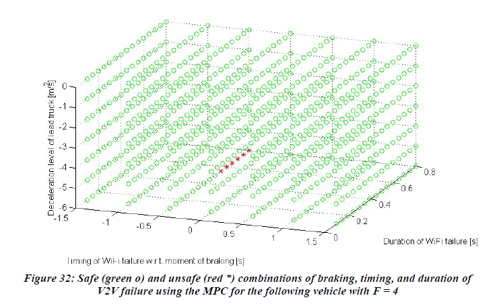
\includegraphics[width=1\columnwidth]{example.png}
  \caption{Example }\label{fig:example}
\end{figure}
